\begin{figure}[t]
    \centering
    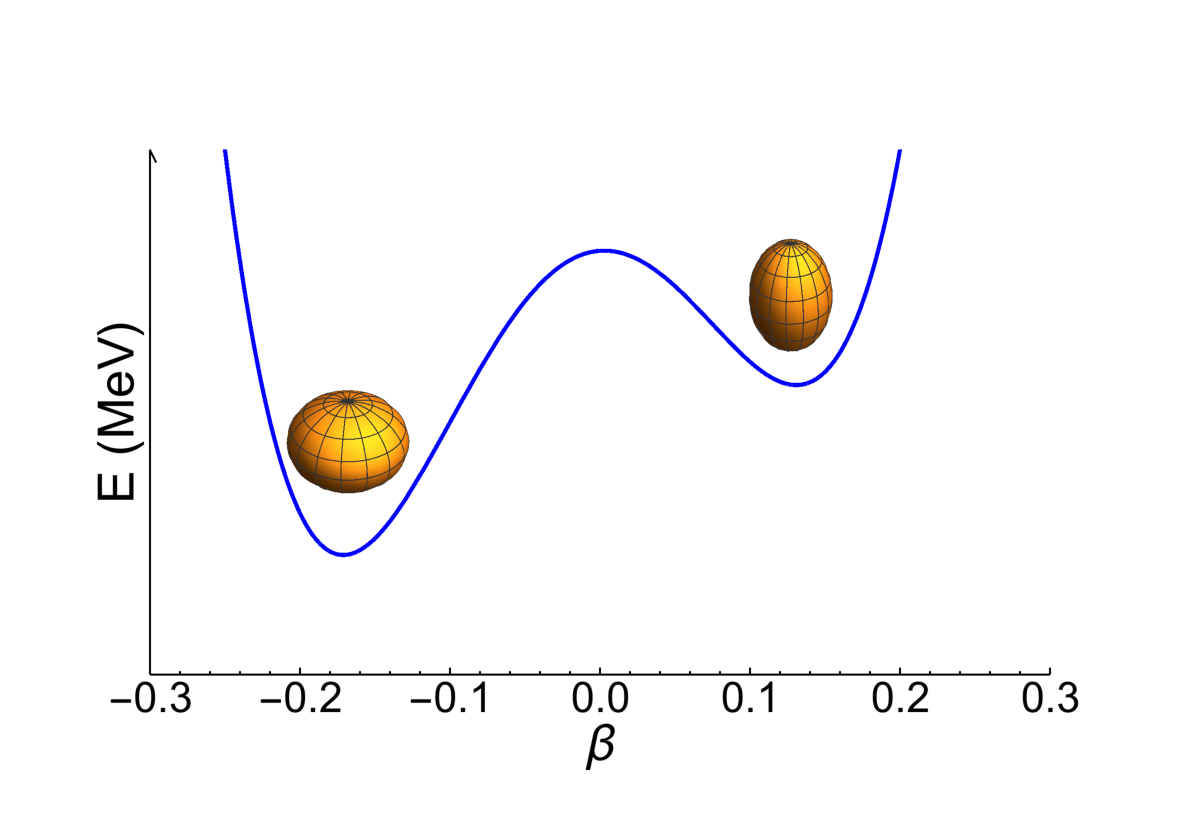
\includegraphics[scale=0.7]{Introduction_Figs/ShapeCoexist.pdf}
    \caption{Cartoon of the potential well of a nucleus with shape coexistence. A second minima appears at a different $\beta$, the deformation parameter. Both of these minima can have excitations built on top of them, leading to shape coexistence. A representation of the shape at $\beta$ is shown in each minima.}
    \label{fig:shape}
\end{figure}